\section{Experimental setup}

\section{Platform and Benchmarks}
We perform our experiments on four ODROID XU3 devices which are a
small mobile devices with Ubuntu 14.04 running on them. The ODROID
boards have Samsung Exynos 5 Octa processors based on the ARM
big.LITTLE architecture.  Each processor has 19 speed settings with
all being available for its 4 big cores and 13 for 4 LITTLE cores.
Each board has a power meter updated at 1 \ms intervals.  Each
resource configuration (combination of big/LITTLE cores and
clockspeeds) has a different performance and power, which is, itself,
application dependent.

We use 20 different benchmarks from five suites including PARSEC
(\texttt{blackscholes},\texttt{facesim}, \texttt{x264} )
\cite{parsec}, Minebench (\texttt{Kmeans}, \texttt{non fuzzy kmeans
  \\* (Kmeansnf)}) \cite{minebench}, Seec (\texttt{dijkstra})
\cite{seec}, Parmibench (\texttt{ferret}) \cite{parmibench}, and
Rodinia
(\texttt{backprop},\texttt{cfd}, \texttt{nn}, \texttt{lud}, \\*
\texttt{backprop}, \texttt{bfs}) \cite{rodinia}.  We also use a
partial differential equation solver (\texttt{jacobi}) and a memory
intensive benchmark pair (\texttt{stream}) and
(\texttt{stream\_threads}) \cite{stream}. Our benchmarks vary from
compute-bound applications to memory bound workloads and also
workloads that are a combination of both as shown in
\figref{application_variety}.  Eachapplication has been instrumented
to report its performance as heartbeats/second an application-specific
performance metric \cite{POET}.

The combination of different types of cores with different clockspeeds
creates a complicated tradeoff space, that is application dependent.
This complexity is one of the reasons to use machine learning to
estimate models.  To demonstrate this complexity we illustrate the
performance and power tradeoff spaces for three example applications
in \figref{fig:contour}.  The figures show cores on the x-axis and
clockspeed on the y-axis performance and power are shown as intensity,
with darker colors representing larger performance/power.

The presence of local minima and maxima mean that simple gradient
ascent/descent methods are not suitable to navigating these tradeoff
spaces. \figref{fig:contour} shows that the performance plot for the
applications \texttt{Kmeans},\texttt{lavamd} and \texttt{x264} against
the clockspeed and cores is non-convex and contains at least 2 local
minima corresponding to big and LITTLE cores.  Similarly, the power
plot for the applications and the surface is non-smooth.  This
non-smoothness is the reason why parametric models of these curves do
not perform well and the hierarchical Bayesian model -- which is
non-parametric -- is not affected by the shape of the curve.

\subsection{Evaluation metrics}
\PUNT{
We evaluate learning methods by computing the \emph{accuracy} of the
learned models:
\begin{equation}
\label{eq:accuracy}
accuracy(\hat{\y},\y) = max\left(1 - \frac{\| \hat{\y}-\y \|^2_2 }{\| \y - \bar{\y}\|^2_2},0\right).
\end{equation}
where $\hat{\y}$ represents the predicted performance/power values
and $\y$ is the true value of the power and performance.
}

\SYSTEM{} uses the model for power and performance and its controller
actively uses this knowledge to meet the performance target. A
performance target can be thought of as a quality of service
expectation for the given application. We run our applications from
10\% to 90\% performance targets and observe how \SYSTEM{} performs
under each constraint. We quantify the ability to meet performance
targets using the standard metric \emph{mean absolute percentage
  error} (MAPE).  Suppose the application wants to emit $n$ heartbeats
while maintaining a speed of $S_r$, then MAPE is calculated as:
\begin{equation}
MAPE = 100\% \cdot \frac{1}{n} \sum\limits_{i=1}^{n} max \left( \frac{S_{r} - s_m(i)}{S_r},0 \right)
\end{equation}
where $S_{r}$ is the performance target and $s_m(i)$ is the
performance observed for $i$th heartbeat.

\begin{figure*}
\centering
%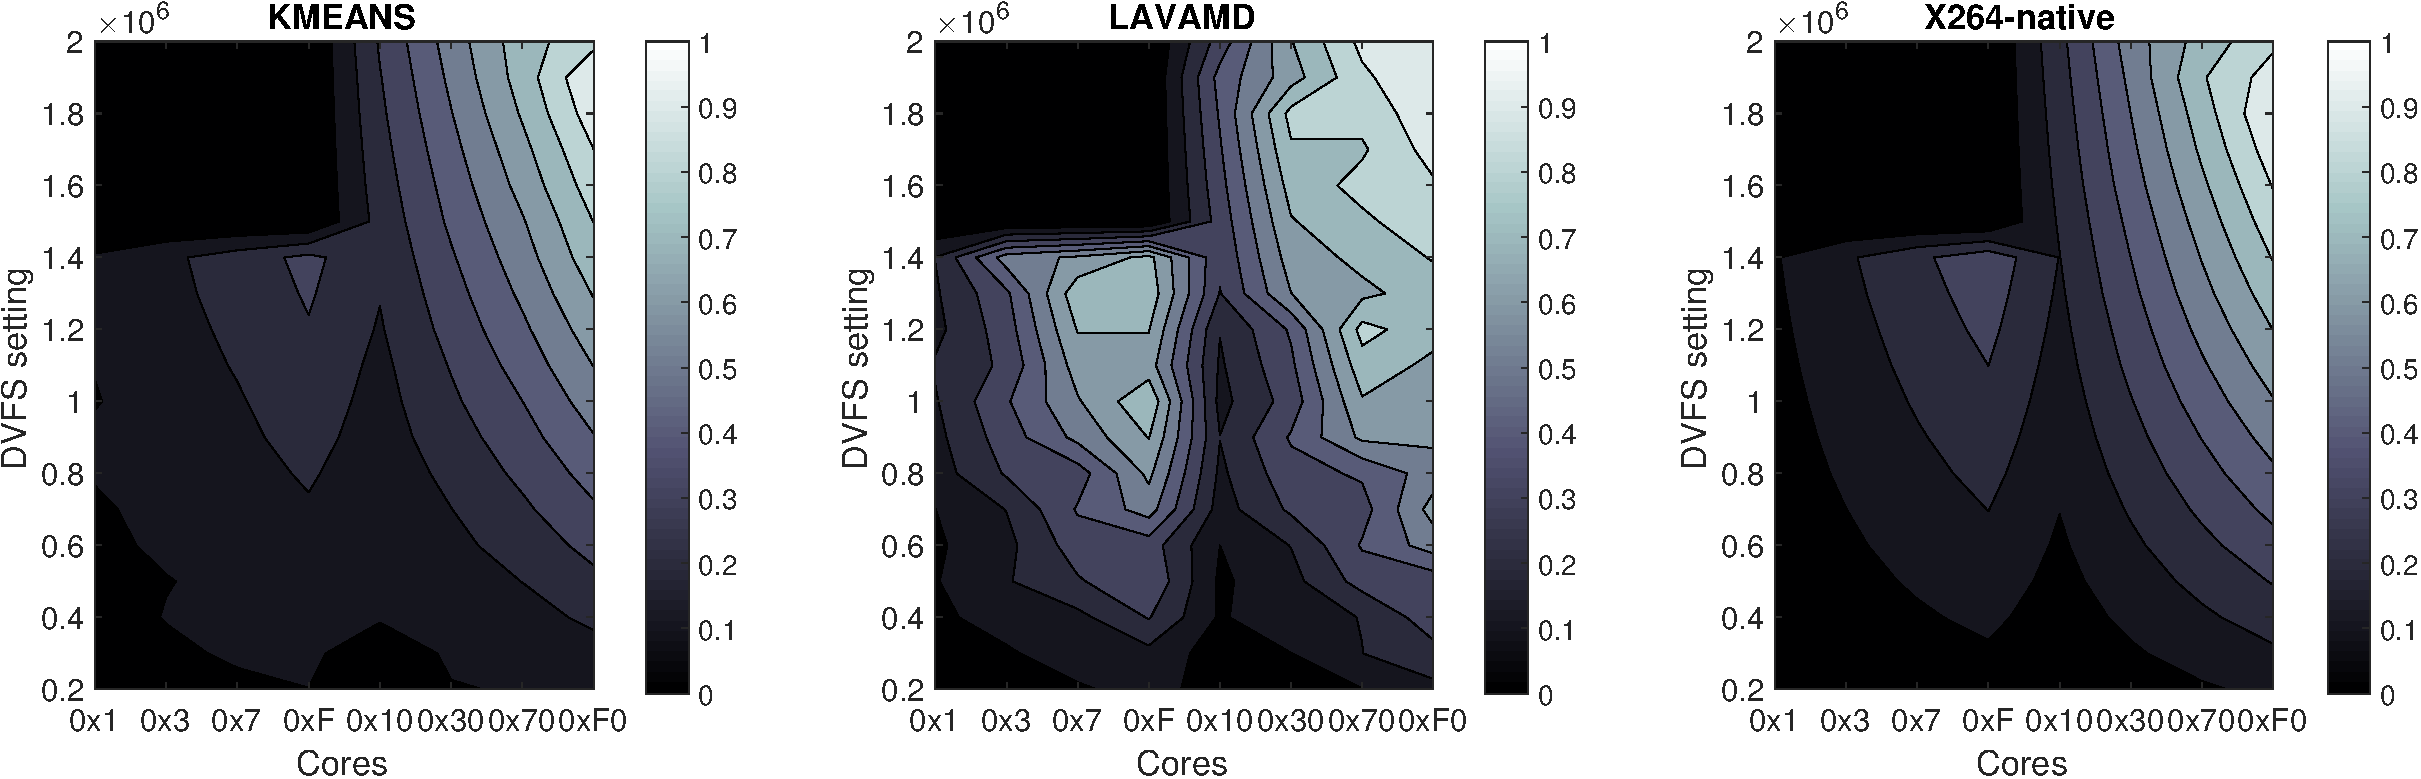
\includegraphics[width=\paperwidth,scale=0.5]{figures/performance-contour3.pdf}
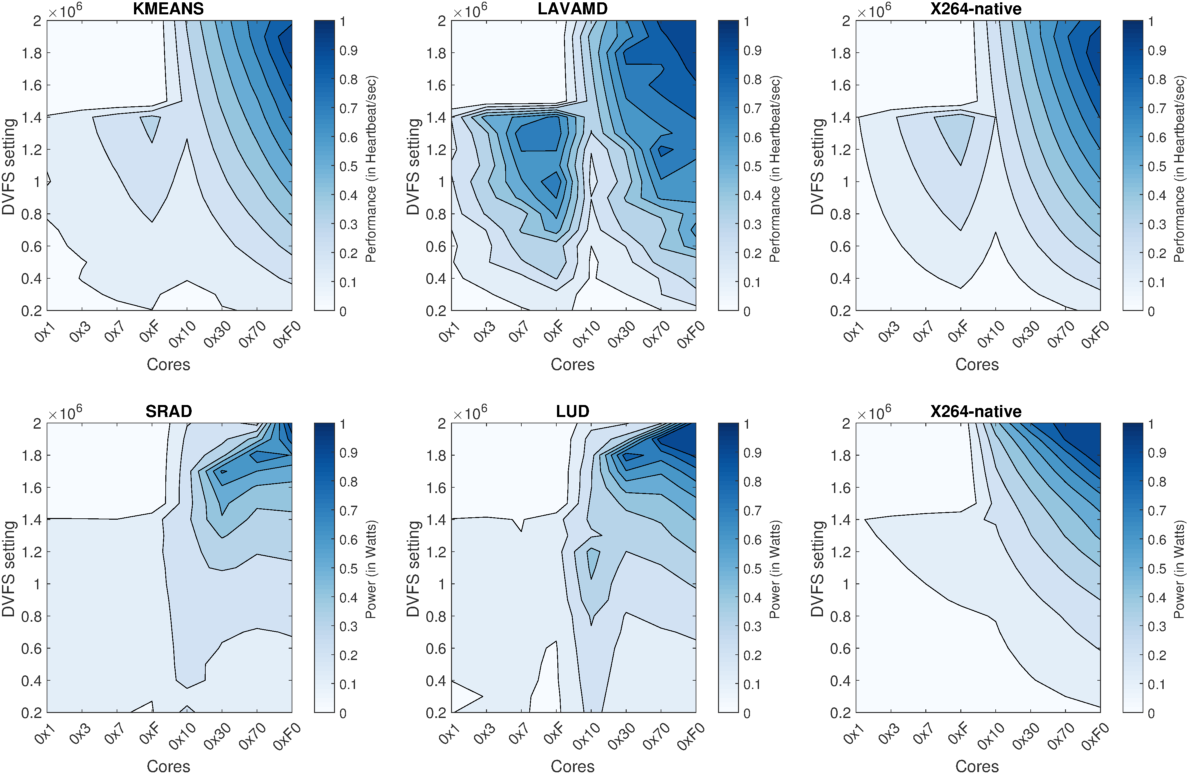
\includegraphics[scale=0.4]{figures/sample-contour3.png}
\caption{Contour.}
  \label{fig:contour}
\end{figure*}

We evaluate energy savings by constructing an oracle.  We run every
application in every resource configuration and record performance and
power for every heartbeat.  By post processing this data we can
determine the optimal configuration for each heartbeat and each
performance target. To produce an energy metric that we can compare
across applications, we normalize energy as:
\begin{equation}
  normalized\,energy = e_m / e_{optimal} - 1
\end{equation}
where $e_m$ is the measured energy and $e_{optimal}$ is the optimal
energy produced by our oracle. We subtract 1, so that this metric
shows the proportion of energy consumed over optimal.  \TODO{Should we
  multiply this by 100, so that it is also a \%?  That seems like a
  good idea -- might as well be consistent across the two metrics.  We
  don't even have to change the data, just the axis labels. }


\subsection{Points of comparison}
As discussed in \secref{learning}, we classify learning approaches
into \emph{Online} and \emph{Offline} approaches, which we then use to
construct baselines to which we compare \SYSTEM{}:
\begin{enumerate}
\item \textit{Online} -- This strategy observes the current
  application in a small number of configurations then performs
  polynomial multivariate regression and estimates the performance and
  power of the unobserrved configurations. \PUNT{Note that the process
    of collecting samples for estimation might be very expensive and
    this model requires a minimum number of samples to start with.
    This method uses only the observations and not the prior data.}
\item \textit{Offline} -- This is our zero-sample policy, used when we
  do not observe any values for the current application. This method
  takes the mean over all known applications and uses that to estimate
  power and performance for new applications.  This strategy only uses
  prior information and does not update the model based on runtime
  observations.
\end{enumerate}

We compare \SYSTEM{}'s combination of HBM with control to baselines
constructed with a combination of different learning models and a
state-of-art controller based on the \emph{Pace-to-idle (P2I)}
heuristic \cite{RACINGPACING}.  Pace-to-idle is proven to be never
worse than race-to-idle and often provides as much as $2\times$
energy savings, but requires application-specific knowledge to
implement.  Pace-to-idle completes jobs in the most energy-efficient
configuration and then transitions to a low-power sleep state until
the next job is ready.  As the energy-efficiency of a configuration is
application-dependent, it is natural to combine pace-to-idle with
machine learning approaches that can estimate the energy efficiency
for different applications.  In the next section, we will compare
\SYSTEM{}'s delivered performance and energy savings with:
\begin{enumerate}
\item \textit{Online-P2I} -- We use the \textit{Online} learning model
  in combination with \emph{Pace-to-idle(P2I)} heuristic.
\item \textit{Offline-P2I} -- We use the \textit{Offline} learning
  model in combination with \emph{Pace-to-idle(P2I)} heuristic.
\item \textit{LEO-P2I} -- We use the \textit{LEO} learning model in
  combination with \emph{Pace-to-idle(P2I)} heuristic.
\item \textit{POET} -- A state-of-the-art, open source control system
  designed to meet application performance with minimal energy.  POET
  requires users to specify a model of resource performance and power
  consumption.  We use POET with the model produced by the
  \emph{Offline} learner.
\end{enumerate}

\section{Experimental Evaluation}
We evaluate \SYSTEM{}'s ability to deliver requested performance with
near-optimal energy.  We first examine performance accuracy and energy
in a single-application scenario, where each application is run by
itself.  We then consider a multi-application scenario where each
application is run and then, halfway through, a second random
application is launched, testing the ability to deliver performance in
a changing environment.  
%We then examine other dynamic scenarios where
%applicaction inputs or behavior changes during application execution.
%Finally we compare the accuracy of the various learning approaches to
%offer insight into why \SYSTEM{} performs so well.

\subsection{Performance and Energy for One App}
%Setup
To test the ability to deliver performance and minimize energy, we set
a range of targets ranging from 10-90\% of the maximum achievable
performance on our system. The extreme targets are generally easy to
hit. The most interesting performance targets are around 30\%-70\%
where there are not obvious choices for configuration settings. These
intermediate targets require a blend of big and LITTLE cores and
getting that blend to both meet the performance and reduce energy is
dependent on accurate models of performance and power.

% Results
The results for these single-application tests are shown in
\figsref{single-perf}{single-energy}.  The benchmarks are shown on the
x-axis; the y-axes show MAPE and the normalized energy, respectively.

We find that \SYSTEM{} has lower MAPE and energy consumption than the
baseline algorithms. Across all applications and targets, the online
model produces an average error of 5.4\%, the offline: 4.4\%, LEO:
4.0\%, POET: 4.7\%, and \SYSTEM{}: 2.0\%.  These results show that
\SYSTEM{} reduces error by a factor of two compared to prior
approaches.  

The energy consumption results are even more impressive.  The online
model requires an average of 30\% more energy than optimal, offline:
16\%, LEO: 20\%, POET: 13\%, and \SYSTEM{}: 5\%.  Thus the combination
of learning and control provides a dramatic reduction in energy
consumption compared to even state-of-the-art learning or control
approaches.  The reason is that the combination is complementary: LEO
produces accurate models while control both can correct small errors
in those models and adapt to dynamic changes in behavior.

\begin{figure*}[t]
  \begin{tikzpicture}
\definecolor{s1}{RGB}{228, 26, 28}
\definecolor{s2}{RGB}{55, 126, 184}
\definecolor{s3}{RGB}{77, 175, 74}
\definecolor{s4}{RGB}{152, 78, 163}
\definecolor{s5}{RGB}{255, 127, 0}

\begin{groupplot}[
    group style={
        group name=plots,
        group size=1 by 5,
        xlabels at=edge top,
        xticklabels at=edge top,
        vertical sep=5pt
    },
axis x line* = top,
xlabel near ticks,
major x tick style = transparent,
height=2.5cm,
width=0.88\textwidth,
xmin=0,
xmax=9,
enlargelimits=false,
tick align = outside,
tick style={white},
ylabel style={align=center},
ytick=\empty,
xtick=\empty,
xticklabels={},
yticklabels={},
ymin=0,
ymax=1,
]
\nextgroupplot[ylabel={$\mathsf{10\%}$},
y label style={rotate=270},
ylabel shift={12mm},
]
\addplot[thick,solid, color=black] coordinates {(0,1) (22,1)};

\nextgroupplot[
ylabel shift={12mm},
y label style={rotate=270},
ylabel={$\mathsf{30\%}$},
]
\addplot[thick,solid, color=black] coordinates {(0,1) (22,1)};

\nextgroupplot[
ylabel shift={12mm},
y label style={rotate=270},
ylabel={$\mathsf{50\%}$},
]
\addplot[thick,solid, color=black] coordinates {(0,1) (22,1)};


\nextgroupplot[
ylabel shift={12mm},
ylabel={$\mathsf{70\%}$},
y label style={rotate=270},
]
\addplot[thick,solid, color=black] coordinates {(0,1) (22,1)};

\nextgroupplot[
ylabel shift={12mm},
ylabel={$\mathsf{90\%}$},
y label style={rotate=270},
]
\addplot[thick,solid, color=black] coordinates {(0,1) (22,1)};

\end{groupplot}

\begin{groupplot}[
    group style={
        group name=plots,
        group size=1 by 5,
        xlabels at=edge bottom,
        xticklabels at=edge bottom,
        vertical sep=5pt
    },
axis x line* = bottom,
xlabel near ticks,
major x tick style = transparent,
xlabel={},
height=2.5cm,
width=0.88\textwidth,
xmin=0,
xmax=22,
enlargelimits=false,
tick align = outside,
tick style={white},
ylabel style={align=center},
ytick=\empty,
ymin=0,
ymax=30,
ytick={0,5,10,15,20},
yticklabels={,5,10,15,20},
legend cell align=left, 
legend style={ column sep=1ex },
ymajorgrids,
grid style={dashed},
]

\nextgroupplot[ybar=\pgflinewidth,
bar width=2.0pt,
legend entries = {{$\mathsf{Online-P2I}$},{$\mathsf{Offline-P2I}$},{$\mathsf{LEO-P2I}$},{$\mathsf{POET}$},{$\mathsf{\SYSTEM{}}$}},
legend style={draw=none,legend columns=5,at={(.5,1.7)},anchor=north},
ylabel shift={0mm},
ymin=0,
ymax=6,
ytick={0.0,2.0,4.0,6.0},
yticklabels={,2.0,4.0,6.0},
]
\addplot table[x index=0,y index=3, col sep=space] {img/image_text/dyn-mape-0.1.txt};
\addplot table[x index=0,y index=4, col sep=space] {img/image_text/dyn-mape-0.1.txt};
\addplot table[x index=0,y index=5, col sep=space] {img/image_text/dyn-mape-0.1.txt};
\addplot table[x index=0,y index=6, col sep=space] {img/image_text/dyn-mape-0.1.txt};
\addplot table[x index=0,y index=7, col sep=space] {img/image_text/dyn-mape-0.1.txt};

\nextgroupplot[ybar=\pgflinewidth,
ylabel shift={0mm},
bar width=2.0pt,
ymin=0,
ymax=20,
ytick={0.0,5.0,10.0,15.0,20.0},
yticklabels={,5.0,10.0,15.0},
]
\addplot table[x index=0,y index=3, col sep=space] {img/image_text/dyn-mape-0.3.txt};
\addplot table[x index=0,y index=4, col sep=space] {img/image_text/dyn-mape-0.3.txt};
\addplot table[x index=0,y index=5, col sep=space] {img/image_text/dyn-mape-0.3.txt};
\addplot table[x index=0,y index=6, col sep=space] {img/image_text/dyn-mape-0.3.txt};
\addplot table[x index=0,y index=7, col sep=space] {img/image_text/dyn-mape-0.3.txt};

\nextgroupplot[ybar=\pgflinewidth,
ylabel={\footnotesize MAPE},
ylabel shift={0mm},
bar width=2.0pt,
ymin=0,
ymax=30,
ytick={0.0,10.0,20.0,30.0},
yticklabels={,10.0,20.0,30.0},
]
\addplot table[x index=0,y index=3, col sep=space] {img/image_text/dyn-mape-0.5.txt};
\addplot table[x index=0,y index=4, col sep=space] {img/image_text/dyn-mape-0.5.txt};
\addplot table[x index=0,y index=5, col sep=space] {img/image_text/dyn-mape-0.5.txt};
\addplot table[x index=0,y index=6, col sep=space] {img/image_text/dyn-mape-0.5.txt};
\addplot table[x index=0,y index=7, col sep=space] {img/image_text/dyn-mape-0.5.txt};

\nextgroupplot[ybar=\pgflinewidth,
ylabel shift={0mm},
bar width=2.0pt,
ymin=0,
ymax=30,
ytick={0.0,10.0,20.0,30.0},
yticklabels={,10.0,20.0,30.0},
]
\addplot table[x index=0,y index=3, col sep=space] {img/image_text/dyn-mape-0.7.txt};
\addplot table[x index=0,y index=4, col sep=space] {img/image_text/dyn-mape-0.7.txt};
\addplot table[x index=0,y index=5, col sep=space] {img/image_text/dyn-mape-0.7.txt};
\addplot table[x index=0,y index=6, col sep=space] {img/image_text/dyn-mape-0.7.txt};
\addplot table[x index=0,y index=7, col sep=space] {img/image_text/dyn-mape-0.7.txt};

\nextgroupplot[ybar=\pgflinewidth,
bar width=2.0pt,
ylabel shift={0mm},
xticklabel shift={0pt},
ymin=0,
ymax=30,
ytick={0.0,10.0,20.0,30.0},
yticklabels={,10.0,20.0,30.0},
x tick label style={rotate=35, anchor=east},
xtick={1,2,3,4,5,6,7,8,9,10,11,12,13,14,15,16,17,18,19,20,21,22},
xticklabels={
{\scriptsize $\mathsf{backprop}$},
{\scriptsize $\mathsf{bfs}$},
{\scriptsize $\mathsf{blackscholes}$},
{\scriptsize $\mathsf{bodytrack}$},
{\scriptsize $\mathsf{facesim}$},
{\scriptsize $\mathsf{ferret}$},
{\scriptsize $\mathsf{heartwall}$},
{\scriptsize $\mathsf{hotspot}$},
{\scriptsize $\mathsf{jacobi}$},
{\scriptsize $\mathsf{kmeans}$},
{\scriptsize $\mathsf{kmeansnf}$},
{\scriptsize $\mathsf{lavamd}$},
{\scriptsize $\mathsf{leukocyte}$},
{\scriptsize $\mathsf{lud}$},
{\scriptsize $\mathsf{nw}$},
{\scriptsize $\mathsf{sha}$},
{\scriptsize $\mathsf{srad}$},
{\scriptsize $\mathsf{stream_threads}$},
{\scriptsize $\mathsf{x264-ducks}$},
{\scriptsize $\mathsf{x264-native}$},
{\scriptsize $\mathsf{\mathbf{Average}}$}},
]
\addplot table[x index=0,y index=3, col sep=space] {img/image_text/dyn-mape-0.9.txt};
\addplot table[x index=0,y index=4, col sep=space] {img/image_text/dyn-mape-0.9.txt};
\addplot table[x index=0,y index=5, col sep=space] {img/image_text/dyn-mape-0.9.txt};
\addplot table[x index=0,y index=6, col sep=space] {img/image_text/dyn-mape-0.9.txt};
\addplot table[x index=0,y index=7, col sep=space] {img/image_text/dyn-mape-0.9.txt};

\end{groupplot}
\end{tikzpicture}
   \vskip -1em
  \caption{Single Applications MAPE}
  \label{fig:single-perf}
\end{figure*}

\begin{figure*}[t]
  \begin{tikzpicture}
\definecolor{s1}{RGB}{228, 26, 28}
\definecolor{s2}{RGB}{55, 126, 184}
\definecolor{s3}{RGB}{77, 175, 74}
\definecolor{s4}{RGB}{152, 78, 163}
\definecolor{s5}{RGB}{255, 127, 0}

\begin{groupplot}[
    group style={
        group name=plots,
        group size=1 by 5,
        xlabels at=edge top,
        xticklabels at=edge top,
        vertical sep=5pt
    },
axis x line* = top,
xlabel near ticks,
major x tick style = transparent,
height=2.5cm,
width=0.88\textwidth,
xmin=0,
xmax=9,
enlargelimits=false,
tick align = outside,
tick style={white},
ylabel style={align=center},
ytick=\empty,
xtick=\empty,
xticklabels={},
yticklabels={},
ymin=0,
ymax=1,
]
\nextgroupplot[ylabel={$\mathsf{10\%}$},
y label style={rotate=270},
ylabel shift={12mm},
]
\addplot[thick,solid, color=black] coordinates {(0,1) (22,1)};
\nextgroupplot[
ylabel shift={12mm},
y label style={rotate=270},
ylabel={$\mathsf{30\%}$},
]
\addplot[thick,solid, color=black] coordinates {(0,1) (22,1)};
\nextgroupplot[
ylabel shift={12mm},
y label style={rotate=270},
ylabel={$\mathsf{50\%}$},
]
\addplot[thick,solid, color=black] coordinates {(0,1) (22,1)};
\nextgroupplot[
ylabel shift={12mm},
ylabel={$\mathsf{70\%}$},
y label style={rotate=270},
]
\addplot[thick,solid, color=black] coordinates {(0,1) (22,1)};
\nextgroupplot[
ylabel shift={12mm},
ylabel={$\mathsf{90\%}$},
y label style={rotate=270},
]
\addplot[thick,solid, color=black] coordinates {(0,1) (22,1)};
\end{groupplot}

\begin{groupplot}[
    group style={
        group name=plots,
        group size=1 by 5,
        xlabels at=edge bottom,
        xticklabels at=edge bottom,
        vertical sep=5pt
    },
axis x line* = bottom,
xlabel near ticks,
major x tick style = transparent,
xlabel={},
height=2.5cm,
width=0.88\textwidth,
xmin=0,
xmax=22,
enlargelimits=false,
tick align = outside,
tick style={white},
ylabel style={align=center},
ytick=\empty,
ymin=0,
ymax=2.5,
ytick={0,0.50,1.50,2.50},
yticklabels={,50,150,250},
legend cell align=left, 
legend style={ column sep=1ex },
ymajorgrids,
grid style={dashed},
]

\nextgroupplot[ybar=\pgflinewidth,
bar width=2.0pt,
legend entries = {{$\mathsf{Online-P2I}$},{$\mathsf{Offline-P2I}$},{$\mathsf{LEO-P2I}$},{$\mathsf{POET}$},{$\mathsf{\SYSTEM{}}$}},
legend style={draw=none,legend columns=5,at={(.5,1.7)},anchor=north},
ylabel shift={0mm},
ymin=0,
ymax=2,
ytick={0,0.5,1.5,2},
yticklabels={,50,150,200},
]
\addplot table[x index=0,y index=3, col sep=space] {img/image_text/dyn-eff-0.1.txt};
\addplot table[x index=0,y index=4, col sep=space] {img/image_text/dyn-eff-0.1.txt};
\addplot table[x index=0,y index=5, col sep=space] {img/image_text/dyn-eff-0.1.txt};
\addplot table[x index=0,y index=6, col sep=space] {img/image_text/dyn-eff-0.1.txt};
\addplot table[x index=0,y index=7, col sep=space] {img/image_text/dyn-eff-0.1.txt};

\nextgroupplot[ybar=\pgflinewidth,
ylabel shift={0mm},
bar width=2.0pt,
%ymin=.9,
%ymax=9,
%ytick={1,2,3,4,5,6,7,8},
%yticklabels={1.0,,,,5.0,,,8.0},
]
\addplot table[x index=0,y index=3, col sep=space] {img/image_text/dyn-eff-0.3.txt};
\addplot table[x index=0,y index=4, col sep=space] {img/image_text/dyn-eff-0.3.txt};
\addplot table[x index=0,y index=5, col sep=space] {img/image_text/dyn-eff-0.3.txt};
\addplot table[x index=0,y index=6, col sep=space] {img/image_text/dyn-eff-0.3.txt};
\addplot table[x index=0,y index=7, col sep=space] {img/image_text/dyn-eff-0.3.txt};

\nextgroupplot[ybar=\pgflinewidth,
ylabel={\footnotesize Normalized energy},
ylabel shift={0mm},
bar width=2.0pt,
%ymin=.9,
%ymax=9,
%ytick={1,2,3,4,5,6,7,8},
%yticklabels={1.0,,,,5.0,,,8.0},
]
\addplot table[x index=0,y index=3, col sep=space] {img/image_text/dyn-eff-0.5.txt};
\addplot table[x index=0,y index=4, col sep=space] {img/image_text/dyn-eff-0.5.txt};
\addplot table[x index=0,y index=5, col sep=space] {img/image_text/dyn-eff-0.5.txt};
\addplot table[x index=0,y index=6, col sep=space] {img/image_text/dyn-eff-0.5.txt};
\addplot table[x index=0,y index=7, col sep=space] {img/image_text/dyn-eff-0.5.txt};

\nextgroupplot[ybar=\pgflinewidth,
ylabel shift={0mm},
bar width=2.0pt,
%ymin=.9,
%ymax=9,
%ytick={1,2,3,4,5,6,7,8},
%yticklabels={1.0,,,,5.0,,,8.0},
ymin=0,
ymax=3,
ytick={0,1,2,3},
yticklabels={,100,200,300},
]
\addplot table[x index=0,y index=3, col sep=space] {img/image_text/dyn-eff-0.7.txt};
\addplot table[x index=0,y index=4, col sep=space] {img/image_text/dyn-eff-0.7.txt};
\addplot table[x index=0,y index=5, col sep=space] {img/image_text/dyn-eff-0.7.txt};
\addplot table[x index=0,y index=6, col sep=space] {img/image_text/dyn-eff-0.7.txt};
\addplot table[x index=0,y index=7, col sep=space] {img/image_text/dyn-eff-0.7.txt};

\nextgroupplot[ybar=\pgflinewidth,
bar width=2.0pt,
ylabel shift={0mm},
xticklabel shift={0pt},
x tick label style={rotate=35, anchor=east},
xtick={1,2,3,4,5,6,7,8,9,10,11,12,13,14,15,16,17,18,19,20,21,22},
ymin=0,
ymax=3.1,
ytick={0,1,2,3},
yticklabels={,100,200,300},
xticklabels={
{\scriptsize $\mathsf{backprop}$},
{\scriptsize $\mathsf{bfs}$},
{\scriptsize $\mathsf{blackscholes}$},
{\scriptsize $\mathsf{bodytrack}$},
{\scriptsize $\mathsf{facesim}$},
{\scriptsize $\mathsf{ferret}$},
{\scriptsize $\mathsf{heartwall}$},
{\scriptsize $\mathsf{hotspot}$},
{\scriptsize $\mathsf{jacobi}$},
{\scriptsize $\mathsf{kmeans}$},
{\scriptsize $\mathsf{kmeansnf}$},
{\scriptsize $\mathsf{lavamd}$},
{\scriptsize $\mathsf{leukocyte}$},
{\scriptsize $\mathsf{lud}$},
{\scriptsize $\mathsf{nw}$},
{\scriptsize $\mathsf{sha}$},
{\scriptsize $\mathsf{srad}$},
{\scriptsize $\mathsf{stream_threads}$},
{\scriptsize $\mathsf{x264-ducks}$},
{\scriptsize $\mathsf{x264-native}$},
{\scriptsize $\mathsf{\mathbf{Average}}$}},
]
\addplot table[x index=0,y index=3, col sep=space] {img/image_text/dyn-eff-0.9.txt};
\addplot table[x index=0,y index=4, col sep=space] {img/image_text/dyn-eff-0.9.txt};
\addplot table[x index=0,y index=5, col sep=space] {img/image_text/dyn-eff-0.9.txt};
\addplot table[x index=0,y index=6, col sep=space] {img/image_text/dyn-eff-0.9.txt};
\addplot table[x index=0,y index=7, col sep=space] {img/image_text/dyn-eff-0.9.txt};

\end{groupplot}
\end{tikzpicture}
   \vskip -1em
  \caption{Single Applications energy}
  \label{fig:single-energy}
\end{figure*}

%In addition to providing better average case behavior, \SYSTEM{}
%provides significantly better worst case behavior.  


\subsection{Performance and Energy for Multile Apps}
In this experiment, we test the ability to deliver performance in an
environment where applications compete for resources.  We launch each
of our benchmarks with a performance target (using the same targets as
the prior study).  Halfway through execution, we start another
application randomly drawn from our benchmark set.  We bind this
application to one big core.  Launching this second application
clearly changes performance and power consumption.  Delivering
performance to the original application in this dynamic scenario
clearly tests the ability to react to environmental changes.

The results for the multi-application tests are shown in
\figsref{multi-perf}{multi-energy}.  The benchmarks are shown on the
x-axis; the y-axes show MAPE and the normalized energy, respectively.
We note that the 90\% target is generally not reachable in this
scenario as it would require the controlled application to have
exclusive use of all big cores.


As in the prior study, \SYSTEM{} has lower MAPE than the baseline
algorithms. Across all applications and targets, the online model
produces an average error of 15\%, the offline: 14\%, LEO: 11\%, POET:
9\%, and \SYSTEM{}: 7\%.  In this case the average numbers skew
\SYSTEM{}'s benefit as no approach does very well with the 90\% target
and all but online do well at the 10\% target.  So, we also consider
worst case behavior for all targets but the 90\% one.  The online
approach has a highest MAPE of 80\% for LUD at the 70\% target.
Offline's highest MAPE is 71\% for STREAM at the 30\% target.  LEO's
highest MAPE is 70\%, also for STREAM at 30\%. POET's highest MAPE of
35\% also occurs for STREAM at 30\%.  \SYSTEM{}'s highest MAPE of 24\%
occurs with LUD at the 70\% target.  POET and \SYSTEM{} both produce
better outcomes in the dynamic scenario because they are specifically
designed to handle system dynamics.  \SYSTEM{}, however, does
significantly better in the worst case than POET because it starts
with better models that are more robust to variation.

The energy consumption results are not as meaningful for this
experiment, but they are included for completeness.  Because there is
another applciation running that is not under control, it consumes
resources and energy that drag down energy efficiency for all
approaches. 

\begin{figure*}[htp!]
  \begin{tikzpicture}
\definecolor{s1}{RGB}{228, 26, 28}
\definecolor{s2}{RGB}{55, 126, 184}
\definecolor{s3}{RGB}{77, 175, 74}
\definecolor{s4}{RGB}{152, 78, 163}
\definecolor{s5}{RGB}{255, 127, 0}

\begin{groupplot}[
    group style={
        group name=plots,
        group size=1 by 5,
        xlabels at=edge top,
        xticklabels at=edge top,
        vertical sep=5pt
    },
axis x line* = top,
xlabel near ticks,
major x tick style = transparent,
height=2.5cm,
width=0.88\textwidth,
xmin=0,
xmax=9,
enlargelimits=false,
tick align = outside,
tick style={white},
ylabel style={align=center},
ytick=\empty,
xtick=\empty,
xticklabels={},
yticklabels={},
ymin=0,
ymax=1,
]
\nextgroupplot[ylabel={$\mathsf{10\%}$},
y label style={rotate=270},
ylabel shift={12mm},
]
\addplot[thick,solid, color=black] coordinates {(0,1) (22,1)};

\nextgroupplot[
ylabel shift={12mm},
y label style={rotate=270},
ylabel={$\mathsf{30\%}$},
]
\addplot[thick,solid, color=black] coordinates {(0,1) (22,1)};

\nextgroupplot[
ylabel shift={12mm},
y label style={rotate=270},
ylabel={$\mathsf{50\%}$},
]
\addplot[thick,solid, color=black] coordinates {(0,1) (22,1)};


\nextgroupplot[
ylabel shift={12mm},
ylabel={$\mathsf{70\%}$},
y label style={rotate=270},
]
\addplot[thick,solid, color=black] coordinates {(0,1) (22,1)};

\nextgroupplot[
ylabel shift={12mm},
ylabel={$\mathsf{90\%}$},
y label style={rotate=270},
]
\addplot[thick,solid, color=black] coordinates {(0,1) (22,1)};

\end{groupplot}

\begin{groupplot}[
    group style={
        group name=plots,
        group size=1 by 5,
        xlabels at=edge bottom,
        xticklabels at=edge bottom,
        vertical sep=5pt
    },
axis x line* = bottom,
xlabel near ticks,
major x tick style = transparent,
xlabel={},
height=2.5cm,
width=0.88\textwidth,
xmin=0,
xmax=22,
enlargelimits=false,
tick align = outside,
tick style={white},
ylabel style={align=center},
ytick=\empty,
ymin=0,
ymax=35,
ytick={0,5,15,25,35},
yticklabels={,5,15,25,35},
legend cell align=left, 
legend style={ column sep=1ex },
ymajorgrids,
grid style={dashed},
]

\nextgroupplot[ybar=\pgflinewidth,
bar width=2.0pt,
legend entries = {{$\mathsf{Online-P2I}$},{$\mathsf{Offline-P2I}$},{$\mathsf{LEO-P2I}$},{$\mathsf{POET}$},{$\mathsf{\SYSTEM{}}$}},
legend style={draw=none,legend columns=5,at={(.5,1.7)},anchor=north},
ylabel shift={0mm},
]
\addplot table[x index=0,y index=2, col sep=space] {img/image_text/ma-err-0.1.txt};
\addplot table[x index=0,y index=3, col sep=space] {img/image_text/ma-err-0.1.txt};
\addplot table[x index=0,y index=4, col sep=space] {img/image_text/ma-err-0.1.txt};
\addplot table[x index=0,y index=5, col sep=space] {img/image_text/ma-err-0.1.txt};
\addplot table[x index=0,y index=6, col sep=space] {img/image_text/ma-err-0.1.txt};

\nextgroupplot[ybar=\pgflinewidth,
ylabel shift={0mm},
bar width=2.0pt,
%ymin=.9,
%ymax=9,
%ytick={1,2,3,4,5,6,7,8},
%yticklabels={1.0,,,,5.0,,,8.0},
]
\addplot table[x index=0,y index=2, col sep=space] {img/image_text/ma-err-0.3.txt};
\addplot table[x index=0,y index=3, col sep=space] {img/image_text/ma-err-0.3.txt};
\addplot table[x index=0,y index=4, col sep=space] {img/image_text/ma-err-0.3.txt};
\addplot table[x index=0,y index=5, col sep=space] {img/image_text/ma-err-0.3.txt};
\addplot table[x index=0,y index=6, col sep=space] {img/image_text/ma-err-0.3.txt};

\nextgroupplot[ybar=\pgflinewidth,
ylabel={\footnotesize MAPE},
ylabel shift={0mm},
bar width=2.0pt,
%ymin=.9,
%ymax=9,
%ytick={1,2,3,4,5,6,7,8},
%yticklabels={1.0,,,,5.0,,,8.0},
]
\addplot table[x index=0,y index=2, col sep=space] {img/image_text/ma-err-0.5.txt};
\addplot table[x index=0,y index=3, col sep=space] {img/image_text/ma-err-0.5.txt};
\addplot table[x index=0,y index=4, col sep=space] {img/image_text/ma-err-0.5.txt};
\addplot table[x index=0,y index=5, col sep=space] {img/image_text/ma-err-0.5.txt};
\addplot table[x index=0,y index=6, col sep=space] {img/image_text/ma-err-0.5.txt};

\nextgroupplot[ybar=\pgflinewidth,
ylabel shift={0mm},
bar width=2.0pt,
%ymin=.9,
%ymax=9,
%ytick={1,2,3,4,5,6,7,8},
%yticklabels={1.0,,,,5.0,,,8.0},
]
\addplot table[x index=0,y index=2, col sep=space] {img/image_text/ma-err-0.7.txt};
\addplot table[x index=0,y index=3, col sep=space] {img/image_text/ma-err-0.7.txt};
\addplot table[x index=0,y index=4, col sep=space] {img/image_text/ma-err-0.7.txt};
\addplot table[x index=0,y index=5, col sep=space] {img/image_text/ma-err-0.7.txt};
\addplot table[x index=0,y index=6, col sep=space] {img/image_text/ma-err-0.7.txt};

\nextgroupplot[ybar=\pgflinewidth,
bar width=2.0pt,
ylabel shift={0mm},
xticklabel shift={0pt},
x tick label style={rotate=35, anchor=east},
xtick={1,2,3,4,5,6,7,8,9,10,11,12,13,14,15,16,17,18,19,20,21,22},
xticklabels={
{\scriptsize $\mathsf{backprop}$},
{\scriptsize $\mathsf{bfs}$},
{\scriptsize $\mathsf{blackscholes}$},
{\scriptsize $\mathsf{bodytrack}$},
{\scriptsize $\mathsf{facesim}$},
{\scriptsize $\mathsf{ferret}$},
{\scriptsize $\mathsf{heartwall}$},
{\scriptsize $\mathsf{hotspot}$},
{\scriptsize $\mathsf{jacobi}$},
{\scriptsize $\mathsf{kmeans}$},
{\scriptsize $\mathsf{kmeansnf}$},
{\scriptsize $\mathsf{lavamd}$},
{\scriptsize $\mathsf{leukocyte}$},
{\scriptsize $\mathsf{lud}$},
{\scriptsize $\mathsf{nw}$},
{\scriptsize $\mathsf{sha}$},
{\scriptsize $\mathsf{srad}$},
{\scriptsize $\mathsf{stream_threads}$},
{\scriptsize $\mathsf{x264-ducks}$},
{\scriptsize $\mathsf{x264-native}$},
{\scriptsize $\mathsf{\mathbf{Average}}$}},
]
\addplot table[x index=0,y index=2, col sep=space] {img/image_text/ma-err-0.9.txt};
\addplot table[x index=0,y index=3, col sep=space] {img/image_text/ma-err-0.9.txt};
\addplot table[x index=0,y index=4, col sep=space] {img/image_text/ma-err-0.9.txt};
\addplot table[x index=0,y index=5, col sep=space] {img/image_text/ma-err-0.9.txt};
\addplot table[x index=0,y index=6, col sep=space] {img/image_text/ma-err-0.9.txt};

\end{groupplot}
\end{tikzpicture}
   \vskip -1em
  \caption{Multi Applications MAPE}
  \label{fig:multi-perf}
\end{figure*}

\begin{figure*}[t]
  \begin{tikzpicture}
\definecolor{s1}{RGB}{228, 26, 28}
\definecolor{s2}{RGB}{55, 126, 184}
\definecolor{s3}{RGB}{77, 175, 74}
\definecolor{s4}{RGB}{152, 78, 163}
\definecolor{s5}{RGB}{255, 127, 0}
\definecolor{s6}{RGB}{239, 159, 0}
\definecolor{s7}{RGB}{86, 180, 233}

\begin{groupplot}[
    group style={
        group name=plots,
        group size=1 by 6,
        xlabels at=edge top,
        xticklabels at=edge top,
        vertical sep=5pt
    },
axis x line* = top,
xlabel near ticks,
major x tick style = transparent,
height=2.5cm,
width=0.88\textwidth,
xmin=0,
xmax=9,
enlargelimits=false,
tick align = outside,
tick style={white},
ylabel style={align=center},
ytick=\empty,
xtick=\empty,
xticklabels={},
yticklabels={},
ymin=0,
ymax=1,
]
\nextgroupplot[ylabel={$\mathsf{40\%}$},
y label style={rotate=270},
ylabel shift={12mm},
]
\addplot[thick,solid, color=black] coordinates {(0,1) (22,1)};

\nextgroupplot[
ylabel shift={12mm},
y label style={rotate=270},
ylabel={$\mathsf{50\%}$},
]
\addplot[thick,solid, color=black] coordinates {(0,1) (22,1)};

\nextgroupplot[
ylabel shift={12mm},
y label style={rotate=270},
ylabel={$\mathsf{60\%}$},
]
\addplot[thick,solid, color=black] coordinates {(0,1) (22,1)};


\nextgroupplot[
ylabel shift={12mm},
ylabel={$\mathsf{70\%}$},
y label style={rotate=270},
]
\addplot[thick,solid, color=black] coordinates {(0,1) (22,1)};

\nextgroupplot[
ylabel shift={12mm},
ylabel={$\mathsf{80\%}$},
y label style={rotate=270},
]
\addplot[thick,solid, color=black] coordinates {(0,1) (22,1)};

\nextgroupplot[
ylabel shift={12mm},
ylabel={$\mathsf{90\%}$},
y label style={rotate=270},
]
\addplot[thick,solid, color=black] coordinates {(0,1) (22,1)};

\end{groupplot}

\begin{groupplot}[
    group style={
        group name=plots,
        group size=1 by 6,
        xlabels at=edge bottom,
        xticklabels at=edge bottom,
        vertical sep=5pt
    },
axis x line* = bottom,
xlabel near ticks,
major x tick style = transparent,
xlabel={},
height=2.5cm,
width=0.88\textwidth,
xmin=0,
xmax=23,
enlargelimits=false,
tick align = outside,
tick style={white},
ylabel style={align=center},
ytick=\empty,
ymin=0.0,
ymax=45.0,
ytick={0.0,15.0,30.0,45.0},
yticklabels={,15.0,30.0,45.0},
legend cell align=left, 
legend style={ column sep=1ex },
ymajorgrids,
grid style={dashed},
]

\nextgroupplot[ybar=\pgflinewidth,
bar width=2.0pt,
legend entries = {{$\mathsf{Online}$},{$\mathsf{Offline}$},{$\mathsf{LEO}$},{$\mathsf{POET}$},{$\mathsf{\SYSTEM{}-NP}$},{$\mathsf{\SYSTEM{}}$}},
legend style={draw=none,legend columns=6,at={(.5,1.7)},anchor=north},
ylabel shift={0mm},
%ymin=0,
%ymax=2,
%ytick={0,50,150,200},
%yticklabels={,50,150,200},
]

\addplot table[x index=0,y index=3, col sep=space] {img/image_text/ma-eff-0.4-v2.txt};
\addplot table[x index=0,y index=4, col sep=space] {img/image_text/ma-eff-0.4-v2.txt};
\addplot table[x index=0,y index=5, col sep=space] {img/image_text/ma-eff-0.4-v2.txt};
\addplot table[x index=0,y index=6, col sep=space] {img/image_text/ma-eff-0.4-v2.txt};
\addplot table[x index=0,y index=7, col sep=space] {img/image_text/ma-eff-0.4-v2.txt};
\addplot table[x index=0,y index=8, col sep=space] {img/image_text/ma-eff-0.4-v2.txt};


\nextgroupplot[ybar=\pgflinewidth,
ylabel shift={0mm},
bar width=2.0pt,
%ymin=0,
%ymax=20,
%ytick={0.0,5.0,10.0,15.0,20.0},
%yticklabels={,5.0,10.0,15.0},
]

\addplot table[x index=0,y index=3, col sep=space] {img/image_text/ma-eff-0.5-v2.txt};
\addplot table[x index=0,y index=4, col sep=space] {img/image_text/ma-eff-0.5-v2.txt};
\addplot table[x index=0,y index=5, col sep=space] {img/image_text/ma-eff-0.5-v2.txt};
\addplot table[x index=0,y index=6, col sep=space] {img/image_text/ma-eff-0.5-v2.txt};
\addplot table[x index=0,y index=7, col sep=space] {img/image_text/ma-eff-0.5-v2.txt};
\addplot table[x index=0,y index=8, col sep=space] {img/image_text/ma-eff-0.5-v2.txt};

\nextgroupplot[ybar=\pgflinewidth,
ylabel={\footnotesize MAPE},
ylabel shift={0mm},
bar width=2.0pt,
%ymin=0,
%ymax=30,
%ytick={0.0,10.0,20.0,30.0},
%yticklabels={,10.0,20.0,30.0},
]

\addplot table[x index=0,y index=3, col sep=space] {img/image_text/ma-eff-0.6-v2.txt};
\addplot table[x index=0,y index=4, col sep=space] {img/image_text/ma-eff-0.6-v2.txt};
\addplot table[x index=0,y index=5, col sep=space] {img/image_text/ma-eff-0.6-v2.txt};
\addplot table[x index=0,y index=6, col sep=space] {img/image_text/ma-eff-0.6-v2.txt};
\addplot table[x index=0,y index=7, col sep=space] {img/image_text/ma-eff-0.6-v2.txt};
\addplot table[x index=0,y index=8, col sep=space] {img/image_text/ma-eff-0.6-v2.txt};

\nextgroupplot[ybar=\pgflinewidth,
ylabel shift={0mm},
bar width=2.0pt,
%ymin=0,
%ymax=30,
%ytick={0.0,10.0,20.0,30.0},
%yticklabels={,10.0,20.0,30.0},
]

\addplot table[x index=0,y index=3, col sep=space] {img/image_text/ma-eff-0.7-v2.txt};
\addplot table[x index=0,y index=4, col sep=space] {img/image_text/ma-eff-0.7-v2.txt};
\addplot table[x index=0,y index=5, col sep=space] {img/image_text/ma-eff-0.7-v2.txt};
\addplot table[x index=0,y index=6, col sep=space] {img/image_text/ma-eff-0.7-v2.txt};
\addplot table[x index=0,y index=7, col sep=space] {img/image_text/ma-eff-0.7-v2.txt};
\addplot table[x index=0,y index=8, col sep=space] {img/image_text/ma-eff-0.7-v2.txt};

\nextgroupplot[ybar=\pgflinewidth,
ylabel shift={0mm},
bar width=2.0pt,
%ymin=0,
%ymax=45,
%ytick={0,15,30,45},
%yticklabels={,15,30,45},
]

\addplot table[x index=0,y index=3, col sep=space] {img/image_text/ma-eff-0.8-v2.txt};
\addplot table[x index=0,y index=4, col sep=space] {img/image_text/ma-eff-0.8-v2.txt};
\addplot table[x index=0,y index=5, col sep=space] {img/image_text/ma-eff-0.8-v2.txt};
\addplot table[x index=0,y index=6, col sep=space] {img/image_text/ma-eff-0.8-v2.txt};
\addplot table[x index=0,y index=7, col sep=space] {img/image_text/ma-eff-0.8-v2.txt};
\addplot table[x index=0,y index=8, col sep=space] {img/image_text/ma-eff-0.8-v2.txt};

\nextgroupplot[ybar=\pgflinewidth,
bar width=2.0pt,
ylabel shift={0mm},
xticklabel shift={0pt},
%ymin=0,
%ymax=45,
%ytick={0,15,30,45},
%yticklabels={,15,30,45},
x tick label style={rotate=35, anchor=east},
xtick={1,2,3,4,5,6,7,8,9,10,11,12,13,14,15,16,17,18,19,20,21,22},
xticklabels={
{\scriptsize $\mathsf{backprop}$},
{\scriptsize $\mathsf{bfs}$},
{\scriptsize $\mathsf{blackscholes}$},
{\scriptsize $\mathsf{bodytrack}$},
{\scriptsize $\mathsf{facesim}$},
{\scriptsize $\mathsf{ferret}$},
{\scriptsize $\mathsf{heartwall}$},
{\scriptsize $\mathsf{hotspot}$},
{\scriptsize $\mathsf{jacobi}$},
{\scriptsize $\mathsf{kmeans}$},
{\scriptsize $\mathsf{kmeansnf}$},
{\scriptsize $\mathsf{lavamd}$},
{\scriptsize $\mathsf{leukocyte}$},
{\scriptsize $\mathsf{lud}$},
{\scriptsize $\mathsf{nw}$},
{\scriptsize $\mathsf{sha}$},
{\scriptsize $\mathsf{srad}$},
{\scriptsize $\mathsf{stream}$},
{\scriptsize $\mathsf{stream_threads}$},
{\scriptsize $\mathsf{x264-ducks}$},
{\scriptsize $\mathsf{x264-native}$},
{\scriptsize $\mathsf{\mathbf{Average}}$}},
]

\addplot table[x index=0,y index=3, col sep=space] {img/image_text/ma-eff-0.9-v2.txt};
\addplot table[x index=0,y index=4, col sep=space] {img/image_text/ma-eff-0.9-v2.txt};
\addplot table[x index=0,y index=5, col sep=space] {img/image_text/ma-eff-0.9-v2.txt};
\addplot table[x index=0,y index=6, col sep=space] {img/image_text/ma-eff-0.9-v2.txt};
\addplot table[x index=0,y index=7, col sep=space] {img/image_text/ma-eff-0.9-v2.txt};
\addplot table[x index=0,y index=8, col sep=space] {img/image_text/ma-eff-0.9-v2.txt};

\end{groupplot}
\end{tikzpicture}
   \vskip -1em
  \caption{Multi Applications Energy}
  \label{fig:multi-energy}
\end{figure*}

To demonstrate the benefits of \SYSTEM{} in this dynamic environment
we look at the specific example of \texttt{bodytrack} at the 70\%
performance target.  The time series data for bodytrack is shown in
\figref{bodytrack-multiapp}.  The figures show time (measured in
frames) on the x-axis and performance/power on the y-axes.
Performance is normalized to the target.  There is a curve for each of
LEO, POET, and \SYSTEM{}.  

\begin{figure}[t]
  \begin{tikzpicture}
\begin{centering}


\begin{groupplot}[
    group style={
        group name=plots,
        group size=1 by 2,
        xlabels at=edge bottom,
        xticklabels at=edge bottom,
        vertical sep=5pt
    },
height=3.5cm,
width=0.95\columnwidth,
xmajorgrids,
ymajorgrids,
grid style={dashed},
xmin=0,
xmax=260,
yticklabel pos=left,
enlargelimits=false,
tick align = outside,
tick style={white},
xticklabel shift={-5pt},
yticklabel shift={-5pt},
ylabel shift={-2pt},
ylabel style={align=center},
unbounded coords=jump,
]

\nextgroupplot[ylabel={\footnotesize Performance \\ (Normalized)}, % Performance
ytick={0.0,0.5,1.0,1.5,2.0},
yticklabels={,0.5,1.0,1.5,2.0},
yticklabel style={font=\footnotesize},
ymin=0,
ymax=1.5,
legend entries={{$\mathsf{POET}$},{$\mathsf{LEO}$},{{$\mathsf{\SYSTEM{}}$}}},
legend style={draw=none,at={(0.5,1.4)},anchor=north,legend columns=4,line width=5pt},
]

\addplot[thick, solid, color=poet, mark=none,each nth point=5] table[x index=0,y index=1,col sep=space] {img/bodytrack/poet2-BODYTRACK.txt};
\addplot[thick, solid, color=leo, mark=none,each nth point=5] table[x index=0,y index=1,col sep=space] {img/bodytrack/leo2-BODYTRACK.txt};
\addplot[thick, solid, color=cal, mark=none,each nth point=5] table[x index=0,y index=1,col sep=space] {img/bodytrack/leopoet2-BODYTRACK.txt};
\addplot[thick, dashed, black] coordinates {(130,0) (130, 2)};

\nextgroupplot[ylabel={\footnotesize Power \\ (Watts)}, % Power
ytick={2.0,4.0,6.0},
yticklabels={0.0,2.0,4.0,6.0},
yticklabel style={font=\footnotesize},
ymin=0,
ymax=6.0,
xlabel={\footnotesize $time$ [frame]},
xlabel near ticks,
]
\addplot[thick, solid, color=poet, mark=none,each nth point=5] table[x index=0,y index=2,col sep=space] {img/bodytrack/poet2-BODYTRACK.txt};
\addplot[thick, solid, color=leo, mark=none,each nth point=5] table[x index=0,y index=2,col sep=space] {img/bodytrack/leo2-BODYTRACK.txt};
\addplot[thick, solid, color=cal, mark=none,each nth point=5] table[x index=0,y index=2,col sep=space] {img/bodytrack/leopoet2-BODYTRACK.txt};
\addplot[thick, dashed, black] coordinates {(130,0) (130, 6)};
\end{groupplot}
\end{centering}

\end{tikzpicture}

   \vskip -1em
  \caption{bodytrack multiapp}
  \label{fig:bodytrack-multiapp}
\end{figure}

This small example clearly illustrates the benefits of \SYSTEM{}
compared to prior approaches that use only control or learning.  There
are two key regions in the figures, the times before the second
application starts (on the left of the vertical dashed line) and the
times after (on the right).  Before the second application starts (at
the dashed line), both LEO and \SYSTEM{} do a good job of tracking the
target and keeping energy low.  In contrast, POET produces oscillating
performance (and thus power) because it has a bad model of LITTLE core
performance causing it to use the LITTLE cores too much and then too
little.  This oscillation also results in unnecessary power
consumption.  After the second application starts, POET and \SYSTEM{}
recognize the performacne has changed and adjust resource usage.
\SYSTEM{} does a slightly better job of tracking the change, producing
fewer oscillations.  LEO cannot adjust to the change as it computes
the optimal configuration once at the beginning of the application.
Overall, LEO produces a MAPE of 13\%, POET's is 9\%, and \SYSTEM{}'s
is 4\%.  \SYSTEM{} produces better results than LEO because it reacts
to the change; it produces better results than POET because it has
captured the complex behavior specific to this application on this
system.

\PUNT{
\subsection{Power and performance estimation}
We use LEO as described in \secref{sec:framework:HBM} to estimate the
power and performance for the applications using only 10 out of 128
observations.

Our results are summarized in \figref{fig:accuracy}. LEO is 13.4\%
better than online and 19.1\% better than offline in terms of
performance estimation and LEO is 3.7\% better than online and 1.5\%
better than offline in terms of power estimation, on average over all
the benchmarks.
%Infact, LEO uniformly performs well for all applications with the worst accuracy being YY as compared to offline and online algorithm.


\begin{figure*}[t]
  \begin{tikzpicture}
\definecolor{s1}{RGB}{228, 26, 28}
\definecolor{s2}{RGB}{55, 126, 184}
\definecolor{s3}{RGB}{77, 175, 74}
\definecolor{s4}{RGB}{152, 78, 163}
\definecolor{s5}{RGB}{255, 127, 0}

\begin{groupplot}[
    group style={
        group name=plots,
        group size=1 by 1,
        xlabels at=edge top,
        xticklabels at=edge top,
        vertical sep=5pt
    },
axis x line* = top,
xlabel near ticks,
major x tick style = transparent,
height=3cm,
width=0.88\textwidth,
xmin=0,
xmax=9,
enlargelimits=false,
tick align = outside,
tick style={white},
ylabel style={align=center},
ytick=\empty,
xtick=\empty,
xticklabels={},
yticklabels={},
ymin=0,
ymax=1,
]
\nextgroupplot[ylabel={},
y label style={rotate=270},
ylabel shift={12mm},
]
\addplot[thick,solid, color=black] coordinates {(0,1) (22,1)};

\nextgroupplot[
ylabel shift={12mm},
y label style={rotate=270},
ylabel={$\mathsf{30\%}$},
]
\addplot[thick,solid, color=black] coordinates {(0,1) (22,1)};

\nextgroupplot[
ylabel shift={12mm},
y label style={rotate=270},
ylabel={$\mathsf{50\%}$},
]
\addplot[thick,solid, color=black] coordinates {(0,1) (22,1)};


\nextgroupplot[
ylabel shift={12mm},
ylabel={$\mathsf{70\%}$},
y label style={rotate=270},
]
\addplot[thick,solid, color=black] coordinates {(0,1) (22,1)};

\nextgroupplot[
ylabel shift={12mm},
ylabel={$\mathsf{90\%}$},
y label style={rotate=270},
]
\addplot[thick,solid, color=black] coordinates {(0,1) (22,1)};

\end{groupplot}

\begin{groupplot}[
    group style={
        group name=plots,
        group size=1 by 2,
        xlabels at=edge bottom,
        xticklabels at=edge bottom,
        vertical sep=5pt
    },
axis x line* = bottom,
xlabel near ticks,
major x tick style = transparent,
xlabel={},
height=3cm,
width=0.88\textwidth,
xmin=0,
xmax=22,
enlargelimits=false,
tick align = outside,
tick style={white},
ylabel style={align=center},
ytick=\empty,
ymin=0,
ymax=1.1,
ytick={0,0.3,0.6,0.9},
yticklabels={,0.3,0.6,0.9},
legend cell align=left, 
legend style={ column sep=1ex },
ymajorgrids,
grid style={dashed},
]


\nextgroupplot[ybar=\pgflinewidth,
bar width=2.0pt,
legend entries = {{$\mathsf{Online}$},{$\mathsf{Offline}$},{$\mathsf{LEO}$}},
legend style={draw=none,legend columns=3,at={(.5,1.7)},anchor=north},
ylabel={\footnotesize Accuracy\\ (Performance)}, 
ylabel shift={0mm},
]
\addplot table[x index=0,y index=5, col sep=space] {img/image_text/accuracy.txt};
\addplot table[x index=0,y index=7, col sep=space] {img/image_text/accuracy.txt};
\addplot table[x index=0,y index=3, col sep=space] {img/image_text/accuracy.txt};

\nextgroupplot[ybar=\pgflinewidth,
bar width=2.0pt,
ylabel={\footnotesize Accuracy\\ (Power)}, 
ylabel shift={0mm},
xticklabel shift={0pt},
x tick label style={rotate=35, anchor=east},
xtick={1,2,3,4,5,6,7,8,9,10,11,12,13,14,15,16,17,18,19,20,21,22},
xticklabels={
{\scriptsize $\mathsf{backprop}$},
{\scriptsize $\mathsf{bfs}$},
{\scriptsize $\mathsf{blackscholes}$},
{\scriptsize $\mathsf{bodytrack}$},
{\scriptsize $\mathsf{facesim}$},
{\scriptsize $\mathsf{ferret}$},
{\scriptsize $\mathsf{heartwall}$},
{\scriptsize $\mathsf{hotspot}$},
{\scriptsize $\mathsf{jacobi}$},
{\scriptsize $\mathsf{kmeans}$},
{\scriptsize $\mathsf{kmeansnf}$},
{\scriptsize $\mathsf{lavamd}$},
{\scriptsize $\mathsf{leukocyte}$},
{\scriptsize $\mathsf{lud}$},
{\scriptsize $\mathsf{nw}$},
{\scriptsize $\mathsf{sha}$},
{\scriptsize $\mathsf{srad}$},
{\scriptsize $\mathsf{stream_threads}$},
{\scriptsize $\mathsf{x264-ducks}$},
{\scriptsize $\mathsf{x264-native}$},
{\scriptsize $\mathsf{\mathbf{Average}}$}},
]
\addplot table[x index=0,y index=4, col sep=space] {img/image_text/accuracy.txt};
\addplot table[x index=0,y index=6, col sep=space] {img/image_text/accuracy.txt};
\addplot table[x index=0,y index=2, col sep=space] {img/image_text/accuracy.txt};

\end{groupplot}
\end{tikzpicture}
   \vskip -1em
  \caption{Accuracy performance}
  \label{fig:accuracy}
\end{figure*}
}

\subsection{Sensitivity to the measured samples}
We examine \SYSTEM{}' sensitivity to sample size.  We vary the number
of samples taken online and show how that affects the accuracy of the
learned models.  We note that this is simply the HBM's accuracy in
producing the model used by the controller.  This number is
significant, because we do not want to take a large number of samples
of new applications, if we can avoid it.

\figref{sensitivity} shows the results and compares \SYSTEM{}'s
accuracy to the online approach for learning both performance (top)
and power (bottom).  The figure shows sample size on the x-axis and
accuracy on the y-axis.  \SYSTEM{}'s HBM initially performs as well as
the Offline approach and as sample size increases, the accuracy
uniformly improves and reaches greater than 90\% with around 20
samples. On the other hand, the online approach needs at least 9
samples so that the design matrix for the polynomial regression has
more samples than variables.  As we get more samples the accuracy for
the online model improves but still does not meet \SYSTEM{}'s accuracy
for the same number of samples.

\begin{figure}[t]
  \begin{tikzpicture}
\begin{centering}

\definecolor{s1}{RGB}{228, 26, 28}
\definecolor{s2}{RGB}{55, 126, 184}
\definecolor{s3}{RGB}{77, 175, 74}
\definecolor{s4}{RGB}{152, 78, 163}
\definecolor{s5}{RGB}{255, 127, 0}

\begin{groupplot}[
    group style={
        group name=plots,
        group size=1 by 2,
        xlabels at=edge bottom,
        xticklabels at=edge bottom,
        vertical sep=5pt
    },
height=3.5cm,
width=0.95\columnwidth,
xmajorgrids,
ymajorgrids,
grid style={dashed},
xmin=0,
xmax=100,
yticklabel pos=left,
enlargelimits=false,
tick align = outside,
tick style={white},
xticklabel shift={-5pt},
yticklabel shift={-5pt},
ylabel shift={-2pt},
ylabel style={align=center},
unbounded coords=jump,
]

\nextgroupplot[ylabel={\footnotesize Accuracy\\(Performance)}, % Performance
xtick={0,20,40,60,80,100},
ytick={0.0,0.3,0.6,0.9,1.0},
yticklabels={,0.3,0.6,0.9,1.0},
yticklabel style={font=\footnotesize},
ymin=0,
ymax=1,
legend entries={{$\mathsf{Online}$},{$\mathsf{\SYSTEM{}}$}},
legend style={draw=none,at={(0.5,1.4)},anchor=north,legend columns=4,line width=5pt},
]
%\addplot[thick, solid, color=s3] table[x index=0,y index=1,col sep=tab] {img/old/x264-phases-clover-dvfs.txt};

\addplot[thick, solid, color=s4] table[x index=0,y index=3,col sep=tab] {img/sample_accuracy.txt};
\addplot[thick, solid, color=s3] table[x index=0,y index=1,col sep=tab] {img/sample_accuracy.txt};
%\addplot[thick, solid, black] coordinates {(0, 1) (4500, 1)};
%\addplot[thick, dashed, black] coordinates {(1500,0) (1500, 2)};
%\addplot[thick, dashed, black] coordinates {(3000,0) (3000, 2)};


\nextgroupplot[ylabel={\footnotesize Accuracy\\ (Power)}, % Power
ytick={0.0,0.3,0.6,0.9,1.0},
yticklabels={,0.3,0.6,0.9,1.0},
yticklabel style={font=\footnotesize},
ymin=0,
ymax=1,
xlabel={\footnotesize \% Samples for training},
xlabel near ticks,
xtick={0,20,40,60,80,100},
xticklabels={0,20,40,60,80,100},
xticklabel style={font=\footnotesize},
]

\addplot[thick, solid, color=s4] table[x index=0,y index=4,col sep=tab] {img/sample_accuracy.txt};
\addplot[thick, solid, color=s3] table[x index=0,y index=2,col sep=tab] {img/sample_accuracy.txt};
%\addplot[thick, dashed, black] coordinates {(1500,0) (1500, 250)};
%\addplot[thick, dashed, black] coordinates {(3000,0) (3000, 250)};

\end{groupplot}
\end{centering}

\end{tikzpicture}

   \vskip -1em
  \caption{Estimation accuracy versus sample size.}
  \label{fig:sensitivity}
\end{figure}

\PUNT{
\subsubsection{Phase change}
In this experiment we demonstrate that \SYSTEM{} allows applications
to operate well by changing resource allotment even if the input to
the application is changing with time. In
\figref{fig:x264-phase-change} we see \texttt{X264}, a video encoder
application runs in 2 different phases with phase change at $180^{th}$
frame. The video encode is running difficult scenes in phase 1 and the
scene become significantly less hard in phase-2. In phase-1, \SYSTEM{}
and the baseline LEO-P2I seem to have lower MAPE as compared to POET.
At the same time, these two algorithms seem to consume less energy
than POET indicating that POET is operating at a configuration not on
the pareto frontier of power and performance. When we change phase,
\SYSTEM{} and LEO-P2I both algorithms are still able to meet the
performance target with far less fluctuations as compared to POET.
But, \SYSTEM{} provides better energy savings as compared to LEO-P2I.

\begin{figure}[t]
  \begin{tikzpicture}
\begin{centering}

\definecolor{s1}{RGB}{228, 26, 28}
\definecolor{s2}{RGB}{55, 126, 184}
\definecolor{s3}{RGB}{77, 175, 74}
\definecolor{s4}{RGB}{152, 78, 163}
\definecolor{s5}{RGB}{255, 127, 0}

\begin{groupplot}[
    group style={
        group name=plots,
        group size=1 by 2,
        xlabels at=edge bottom,
        xticklabels at=edge bottom,
        vertical sep=5pt
    },
height=3.5cm,
width=0.95\columnwidth,
xmajorgrids,
ymajorgrids,
grid style={dashed},
xmin=0,
xmax=1000,
yticklabel pos=left,
enlargelimits=false,
tick align = outside,
tick style={white},
xticklabel shift={-5pt},
yticklabel shift={-5pt},
ylabel shift={-2pt},
ylabel style={align=center},
unbounded coords=jump,
]

\nextgroupplot[ylabel={\footnotesize Performance \\ (Normalized)}, % Performance
%xtick={0,500,1000,1500,2000,2500,3000,3500,4000,4500},
ytick={0.0,0.5,1.0,1.5,2.0},
yticklabels={,0.5,1.0,1.5,2.0},
%xtick={0,30,60,120,160,200,240,280,320,480},
%xticklabels={,0,30,60,120,160,200,240,280,320,480},
yticklabel style={font=\footnotesize},
ymin=0,
ymax=1.5,
legend entries={{$\mathsf{POET}$},{$\mathsf{LEO}$},{{$\mathsf{\SYSTEM{}}$}}},
legend style={draw=none,at={(0.5,1.4)},anchor=north,legend columns=4,line width=5pt},
]
\addplot[thick, solid, color=s5] table[x index=0,y index=1,col sep=space] {img/x264-native-ducks/poet-x264.txt};
\addplot[thick, solid, color=s4] table[x index=0,y index=1,col sep=space] {img/x264-native-ducks/leo-x264.txt};
\addplot[thick, solid, color=s3] table[x index=0,y index=1,col sep=space] {img/x264-native-ducks/leopoet-x264.txt};

%\addplot[thick, solid, color=s3] table[x index=0,y index=1,col sep=tab] {img/x264-phases-clover-dvfs.txt};
%\addplot[thick, solid, color=s4] table[x index=0,y index=1,col sep=tab] {img/x264-phases-clover-copper.txt};
%\addplot[thick, solid, black] coordinates {(0, 1) (4500, 1)};
\addplot[thick, dashed, black] coordinates {(500,0) (500, 2)};
%\addplot[thick, dashed, black] coordinates {(3000,0) (3000, 2)};


\nextgroupplot[ylabel={\footnotesize Power \\ (Watts)}, % Power
ytick={0.0,1.0,2.0,3.0,4.0},
yticklabels={,1.0,2.0,3.0,4.0},
yticklabel style={font=\footnotesize},
ymin=0,
ymax=5,
xlabel={\footnotesize $time$ [frame]},
xlabel near ticks,
%xtick={0,500,1000,1500,2000,2500,3000,3500,4000,4500},
%xtick={0,30,60,120,160,200,240,280,320,480},
xticklabels={,0,200,400,600,800,1000},
%xticklabel style={font=\footnotesize},
]
\addplot[thick, solid, color=s5] table[x index=0,y index=2,col sep=space] {img/x264-native-ducks/poet-x264.txt};
\addplot[thick, solid, color=s4] table[x index=0,y index=2,col sep=space] {img/x264-native-ducks/leo-x264.txt};
\addplot[thick, solid, color=s3] table[x index=0,y index=2,col sep=space] {img/x264-native-ducks/leopoet-x264.txt};
%\addplot[thick, solid, color=s3] table[x index=0,y index=2,col sep=tab] {img/x264-phases-clover-dvfs.txt};
%\addplot[thick, solid, color=s4] table[x index=0,y index=2,col sep=tab] {img/x264-phases-clover-copper.txt};
%\addplot[thick, dashed, black] coordinates {(1500,0) (1500, 250)};
%\addplot[thick, dashed, black] coordinates {(3000,0) (3000, 250)};
\addplot[thick, dashed, black] coordinates {(500,0) (500, 5)};
\end{groupplot}
\end{centering}

\end{tikzpicture}

   \vskip -1em
  \caption{X264 phase change}
  \label{fig:x264-phase-change}
\end{figure}

\PUNT{
\begin{figure}[t]
  \begin{tikzpicture}
\begin{centering}

\definecolor{s1}{RGB}{228, 26, 28}
\definecolor{s2}{RGB}{55, 126, 184}
\definecolor{s3}{RGB}{77, 175, 74}
\definecolor{s4}{RGB}{152, 78, 163}
\definecolor{s5}{RGB}{255, 127, 0}

\begin{groupplot}[
    group style={
        group name=plots,
        group size=1 by 2,
        xlabels at=edge bottom,
        xticklabels at=edge bottom,
        vertical sep=5pt
    },
height=3.5cm,
width=0.95\columnwidth,
xmajorgrids,
ymajorgrids,
grid style={dashed},
xmin=0,
xmax=260,
yticklabel pos=left,
enlargelimits=false,
tick align = outside,
tick style={white},
xticklabel shift={-5pt},
yticklabel shift={-5pt},
ylabel shift={-2pt},
ylabel style={align=center},
unbounded coords=jump,
]

\nextgroupplot[ylabel={\footnotesize Performance \\ (Normalized)}, % Performance
%xtick={0,500,1000,1500,2000,2500,3000,3500,4000,4500},
ytick={0.0,0.5,1.0,1.5,2.0},
yticklabels={,0.5,1.0,1.5,2.0},
%xtick={0,30,60,120,160,200,240,280,320,480},
%xticklabels={,0,30,60,120,160,200,240,280,320,480},
yticklabel style={font=\footnotesize},
ymin=0,
ymax=1.5,
legend entries={POET,LEO,{{$\mathsf{\SYSTEM{}}$}}},
legend style={draw=none,at={(0.5,1.4)},anchor=north,legend columns=4,line width=5pt},
]

\addplot[thick, solid, color=s5] table[x index=0,y index=1,col sep=space] {img/ferret/poet-FERRET.txt};
\addplot[thick, solid, color=s3] table[x index=0,y index=1,col sep=space] {img/ferret/leo-FERRET.txt};
\addplot[thick, solid, color=s4] table[x index=0,y index=1,col sep=space] {img/ferret/leopoet-FERRET.txt};
\addplot[thick, dashed, black] coordinates {(1000,0) (1000, 2)};

\nextgroupplot[ylabel={\footnotesize Power \\ (Watts)}, % Power
ytick={0.0,1.0,2.0},
yticklabels={,1.0,2.0},
yticklabel style={font=\footnotesize},
ymin=0,
ymax=5,
xlabel={\footnotesize $time$ [frame]},
xlabel near ticks,
%xtick={0,500,1000,1500,2000,2500,3000,3500,4000,4500},
%xtick={0,30,60,120,160,200,240,280,320,480},
xticklabels={,0,60,120,240,360,480},
%xticklabel style={font=\footnotesize},
]
\addplot[thick, solid, color=s5] table[x index=0,y index=2,col sep=space] {img/ferret/poet-FERRET.txt};
\addplot[thick, solid, color=s3] table[x index=0,y index=2,col sep=space] {img/ferret/leo-FERRET.txt};
\addplot[thick, solid, color=s4] table[x index=0,y index=2,col sep=space] {img/ferret/leopoet-FERRET.txt};
\addplot[thick, dashed, black] coordinates {(1000,0) (1000, 2)};
\end{groupplot}
\end{centering}

\end{tikzpicture}

   \vskip -1em
  \caption{ferret multiapp}
  \label{fig:multi-energy}
\end{figure}
}
}

\subsubsection{Overhead}
The main overhead of \SYSTEM{} is due to sampling where the
applications need to run through a few configurations before \SYSTEM{}
can reliably estimate the entire power and performance frontier. We
argue that the sampling cost can be distributed across devices by
asking each of them to contribute samples for estimation. Once the
sampling phase is over, the HBM is quite fast and can generate an
estimate as fast as 500 ms which is significantly smaller than the
time required for sampling the applications. \TODO{Expand on the
  controller overhead.}











